\pdfinfoomitdate=1
\pdftrailerid{}
\pdfsuppressptexinfo=-1
\documentclass[10pt,a4paper]{article}
\usepackage{cmap}
\usepackage[margin=1.8cm,headheight=14pt,headsep=10pt]{geometry}
\usepackage[leqno]{amsmath}
\usepackage{amssymb,booktabs,longtable,array,ragged2e,multicol,multirow,xcolor,fancyhdr,tikz}
\definecolor{linkblue}{rgb}{0.08,0.33,0.58}
\usepackage[colorlinks=true,linkcolor=linkblue,urlcolor=linkblue,citecolor=linkblue,
  filecolor=linkblue,linktoc=all,pdfborder={0 0 0},bookmarksnumbered=true]{hyperref}
\setlength{\parindent}{0pt}\setlength{\parskip}{4pt}
\setcounter{secnumdepth}{2}\setcounter{tocdepth}{2}
\definecolor{partshade}{gray}{0.9}
\definecolor{parttitle}{HTML}{7A1466}
\definecolor{parttitlelight}{HTML}{D66EBC}
\makeatletter
\renewcommand\section{\@startsection{section}{1}{\z@}{-3ex plus -1ex minus -.2ex}%
  {1.2ex plus .2ex}{\normalfont\large\sffamily\bfseries\color{parttitle}}}
\renewcommand\subsection{\@startsection{subsection}{2}{\z@}{-2.5ex plus -1ex minus -.2ex}%
  {.8ex plus .2ex}{\normalfont\sffamily\bfseries\color{parttitle}}}
\renewcommand\subsubsection{\@startsection{subsubsection}{3}{\z@}{-2ex plus -1ex minus -.2ex}%
  {.6ex plus .2ex}{\normalfont\small\sffamily\bfseries\color{parttitle}}}
\renewcommand\paragraph{\@startsection{paragraph}{4}{\z@}{1.5ex plus .5ex minus .2ex}{-1em}%
  {\normalfont\small\sffamily\bfseries\color{parttitle}}}
\renewcommand\tagform@[1]{\maketag@@@{\textsf{\bfseries\footnotesize (#1)}}}
\renewcommand*\l@part[2]{\par\addvspace{1.6ex}\noindent{\sffamily\bfseries #1}\hfill
  {\sffamily\bfseries #2}\par\nobreak}
\newcommand\tocnumber{1.8em}
\newcommand\tocline[4]{\par{\rightskip \tocnumber plus 1fil\relax\parfillskip -\rightskip
  \noindent\hangindent\dimexpr#1+#2\relax\hspace*{#1}%
  \@tempdima #2{\sffamily\small #3}\nobreak\leaders\hbox{$\m@th\mkern 4.5mu\hbox{.}%
  \mkern 4.5mu$}\hfill\nobreak\hbox to \tocnumber{\hfil\sffamily\small #4}\par}}
\renewcommand*\l@section[2]{\tocline{0em}{2.2em}{#1}{#2}}
\renewcommand*\l@subsection[2]{\tocline{2.2em}{2.6em}{#1}{#2}}
\newcommand\contentspage{{\setlength{\columnsep}{24pt}\begin{multicols}{2}\@starttoc{toc}%
  \end{multicols}}}
\newcounter{docpart}\@addtoreset{section}{docpart}
\renewcommand\thesection{\ifnum\value{docpart}>0 \arabic{docpart}.\fi\arabic{section}}
\renewcommand\theHsection{\arabic{docpart}.\arabic{section}}
\newcommand\partnumber[1]{#1\enspace}
\pdfstringdefDisableCommands{\def\partnumber#1{#1 }}
\newcommand{\partbox}[1]{\par\addvspace{12pt}\refstepcounter{docpart}\phantomsection
  \addcontentsline{toc}{part}{\protect\partnumber{\thedocpart}#1}%
  \noindent\colorbox{partshade}{\makebox[%
  \dimexpr\textwidth-2\fboxsep\relax]{\rule[-6pt]{0pt}{20pt}\Large\sffamily\bfseries%
  \textcolor{parttitle}{\thedocpart\quad #1}}}\par\nobreak\@nobreaktrue\addvspace{2pt}}
\newmarks\LTstartmarks\newcount\LTstartcount
\let\LT@startplain\LT@start
\def\LT@start{\global\advance\LTstartcount\@ne\LT@startplain
  \marks\LTstartmarks{\the\LTstartcount}}
\newmarks\LTgroupmarks
\newcount\LTspacebreak\LTspacebreak=-1
\newcount\LTrulebreak\LTrulebreak=-2
\def\grouprule#1#2{\noalign{\marks\LTgroupmarks{\the\belowrulesep}\nobreak\vskip#1%
  \vskip\aboverulesep}\multispan\LT@cols\unskip{\leaders\hrule\@height#2\hfill\kern\z@}\cr
  \noalign{\penalty\LTrulebreak\vskip\belowrulesep\global\@lastruleclass\z@}}
\def\groupspace#1{\noalign{\marks\LTgroupmarks{\the\dimexpr#1\relax}\penalty\LTspacebreak
  \vskip#1\global\@lastruleclass\z@}}
\def\LT@unskips{\unskip\unpenalty\unskip\unpenalty\unskip\unpenalty\unskip\unpenalty}
\def\LT@groupcut{\ifnum\outputpenalty=\LTrulebreak
  \setbox\@cclv\vbox{\unvbox\@cclv\setbox\z@\lastbox\LT@unskips}\fi}
\def\LT@groupjoin{\ifnum\outputpenalty=\LTspacebreak\vskip-\botmarks\LTgroupmarks\relax\fi
  \ifnum\outputpenalty=\LTrulebreak\vskip-\botmarks\LTgroupmarks\relax\fi}
\let\LT@outputplain\LT@output
\def\LT@output{\ifnum\outputpenalty<-\@Mi\LT@outputplain\else
  \edef\LT@marka{\botmarks\LTstartmarks}\edef\LT@markb{\the\LTstartcount}%
  \ifx\LT@marka\LT@markb\LT@groupcut\LT@outputplain\LT@groupjoin
  \else\setbox\LT@head\box\voidb@x\LT@outputplain\fi\fi}
\makeatother
\newcommand{\needspace}[1]{\par\penalty-100\begingroup\dimen0=#1\relax\dimen2=\pagegoal
  \advance\dimen2-\pagetotal\ifdim\dimen0>\dimen2\relax\ifdim\dimen2>0pt\vfil\break\fi\fi
  \endgroup}
\numberwithin{equation}{section}
\pagestyle{fancy}\fancyhf{}
\renewcommand{\headrulewidth}{0pt}
\renewcommand{\sectionmark}[1]{\markright{\thesection\enspace #1}}
\renewcommand{\subsectionmark}[1]{}
\fancyhead[R]{\small\textsc{\rightmark}\quad\thepage}
\fancypagestyle{plain}{\fancyhf{}\fancyfoot[C]{\small\thepage}}
\definecolor{atlasI}{HTML}{991A1A}\definecolor{atlasIl}{HTML}{EC6B60}
\definecolor{atlasII}{HTML}{295A2C}\definecolor{atlasIIl}{HTML}{6C9F6D}
\definecolor{atlasIII}{HTML}{7A1466}\definecolor{atlasIIIl}{HTML}{D66EBC}
\definecolor{atlasIV}{HTML}{9B690B}\definecolor{atlasIVl}{HTML}{F2A618}
\makeatletter
\newcommand\atlas@full{%
\fill[atlasIII] (0.0394,0.0163) -- (0.3978,0.0163) arc[start angle=0.668, end angle=13.836, radius=1.3979] -- cycle;
\fill[atlasI] (-0.0163,0.0394) -- (-0.0163,0.3978) arc[start angle=90.668, end angle=103.836, radius=1.3979] -- cycle;
\fill[atlasIV] (-0.0394,-0.0163) -- (-0.3978,-0.0163) arc[start angle=-179.332, end angle=-166.164, radius=1.3979] -- cycle;
\fill[atlasII] (0.0163,-0.0394) -- (0.0163,-0.3978) arc[start angle=-89.332, end angle=-76.164, radius=1.3979] -- cycle;
\fill[atlasIIIl] (0.0163,0.0394) -- (0.3343,0.3573) arc[start angle=76.164, end angle=89.332, radius=1.3979] -- cycle;
\fill[atlasIl] (-0.0394,0.0163) -- (-0.3573,0.3343) arc[start angle=166.164, end angle=179.332, radius=1.3979] -- cycle;
\fill[atlasIVl] (-0.0163,-0.0394) -- (-0.3343,-0.3573) arc[start angle=-103.836, end angle=-90.668, radius=1.3979] -- cycle;
\fill[atlasIIl] (0.0394,-0.0163) -- (0.3573,-0.3343) arc[start angle=-13.836, end angle=-0.668, radius=1.3979] -- cycle;
\fill[atlasIIIl] (0.4304,0.0163) -- (0.9598,0.0163) arc[start angle=46.637, end angle=73.849, radius=1.3979] arc[start angle=13.862, end angle=0.653, radius=1.4305] -- cycle;
\fill[atlasIl] (-0.0163,0.4304) -- (-0.0163,0.9598) arc[start angle=136.637, end angle=163.849, radius=1.3979] arc[start angle=103.862, end angle=90.653, radius=1.4305] -- cycle;
\fill[atlasIVl] (-0.4304,-0.0163) -- (-0.9598,-0.0163) arc[start angle=-133.363, end angle=-106.151, radius=1.3979] arc[start angle=-166.138, end angle=-179.347, radius=1.4305] -- cycle;
\fill[atlasIIl] (0.0163,-0.4304) -- (0.0163,-0.9598) arc[start angle=-43.363, end angle=-16.151, radius=1.3979] arc[start angle=-76.138, end angle=-89.347, radius=1.4305] -- cycle;
\fill[atlasIII] (0.0163,0.4304) arc[start angle=89.347, end angle=76.138, radius=1.4305] arc[start angle=16.151, end angle=43.363, radius=1.3979] -- cycle;
\fill[atlasI] (-0.4304,0.0163) arc[start angle=179.347, end angle=166.138, radius=1.4305] arc[start angle=106.151, end angle=133.363, radius=1.3979] -- cycle;
\fill[atlasIV] (-0.0163,-0.4304) arc[start angle=-90.653, end angle=-103.862, radius=1.4305] arc[start angle=-163.849, end angle=-136.637, radius=1.3979] -- cycle;
\fill[atlasII] (0.4304,-0.0163) arc[start angle=-0.653, end angle=-13.862, radius=1.4305] arc[start angle=-73.849, end angle=-46.637, radius=1.3979] -- cycle;
\fill[atlasIII] (0.9997,0.0232) arc[start angle=1.329, end angle=44.066, radius=1] -- (0.3973,0.3742) arc[start angle=73.875, end angle=45.664, radius=1.4305] -- cycle;
\fill[atlasI] (-0.0232,0.9997) arc[start angle=91.329, end angle=134.066, radius=1] -- (-0.3742,0.3973) arc[start angle=163.875, end angle=135.664, radius=1.4305] -- cycle;
\fill[atlasIV] (-0.9997,-0.0232) arc[start angle=-178.671, end angle=-135.934, radius=1] -- (-0.3973,-0.3742) arc[start angle=-106.125, end angle=-134.336, radius=1.4305] -- cycle;
\fill[atlasII] (0.0232,-0.9997) arc[start angle=-88.671, end angle=-45.934, radius=1] -- (0.3742,-0.3973) arc[start angle=-16.125, end angle=-44.336, radius=1.4305] -- cycle;
\fill[atlasIIIl] (0.0232,0.9997) arc[start angle=44.336, end angle=16.125, radius=1.4305] -- (0.6955,0.7185) arc[start angle=45.934, end angle=88.671, radius=1] -- cycle;
\fill[atlasIl] (-0.9997,0.0232) arc[start angle=134.336, end angle=106.125, radius=1.4305] -- (-0.7185,0.6955) arc[start angle=135.934, end angle=178.671, radius=1] -- cycle;
\fill[atlasIVl] (-0.0232,-0.9997) arc[start angle=-135.664, end angle=-163.875, radius=1.4305] -- (-0.6955,-0.7185) arc[start angle=-134.066, end angle=-91.329, radius=1] -- cycle;
\fill[atlasIIl] (0.9997,-0.0232) arc[start angle=-45.664, end angle=-73.875, radius=1.4305] -- (0.7185,-0.6955) arc[start angle=-44.066, end angle=-1.329, radius=1] -- cycle;
}
\newcommand\atlas@draw[2]{\begin{tikzpicture}[x=\dimexpr(#1)/2\relax,y=\dimexpr(#1)/2\relax]
\useasboundingbox (-1,-1) rectangle (1,1);#2\end{tikzpicture}}
\newcommand\atlas@volume[1]{{%
\colorlet{atlasI}{parttitle}\colorlet{atlasIl}{parttitlelight}%
\colorlet{atlasII}{parttitle}\colorlet{atlasIIl}{parttitlelight}%
\colorlet{atlasIII}{parttitle}\colorlet{atlasIIIl}{parttitlelight}%
\colorlet{atlasIV}{parttitle}\colorlet{atlasIVl}{parttitlelight}%
#1}}
\newcommand\atlasmark[1]{\atlas@draw{#1}{\atlas@full}}
\newcommand\volumemark[1]{\atlas@volume{\atlasmark{#1}}}
\makeatother
\fancypagestyle{opening}{\fancyhf{}\fancyfoot[C]{\small\thepage}%
  \fancyhead[L]{\smash{\raisebox{-9.5mm}{\volumemark{12mm}}}}}
\hypersetup{pdftitle={O3-1p: Point Group Atlas, volume III: magnetic point groups}, pdfsubject={Point Group Atlas magnetic record O3-1p, schema point-group-atlas/magnetic/group-continuous/1}}
\fancyhead[L]{\small $\grp{O(3)1'}$}
\DeclareMathAlphabet{\mathelt}{OT1}{cmss}{m}{sl}
\DeclareSymbolFont{eltgreek}{OML}{cmssm}{m}{it}
\DeclareMathSymbol{\eltsigma}{\mathord}{eltgreek}{"1B}
\DeclareSymbolFont{eltletters}{OT1}{cmss}{m}{sl}
\DeclareMathSymbol{g}{\mathalpha}{eltletters}{`g}
\DeclareMathSymbol{h}{\mathalpha}{eltletters}{`h}
\DeclareMathSymbol{Q}{\mathalpha}{eltletters}{`Q}
\DeclareMathSymbol{R}{\mathalpha}{eltletters}{`R}
\DeclareMathSymbol{\xi}{\mathord}{eltgreek}{"18}
\newcommand{\eltfont}[1]{{\let\sigma\eltsigma\mathelt{#1}}}
\newcommand{\grp}[1]{\mathsf{#1}}
\newcommand{\irr}[1]{\text{\normalfont\scshape #1}}
\newcommand{\conjpair}[1]{{}^{#1}}
\newcommand{\cls}[1]{\eltfont{#1}}
\newcommand{\comp}[1]{\eltfont{#1}}
\newcommand{\elt}[1]{\eltfont{#1}}
\newcommand{\hmname}[1]{#1}
\newcommand{\orbname}[1]{#1}
\newcommand{\ptag}[1]{\mathrm{#1}}
\newcommand{\dirprod}{\times}
\newcommand{\nconj}[1]{{\scriptsize$\times#1$}}
\newcommand{\clsletter}[1]{\,{\scriptsize\color{black!55}#1}}
\newcommand{\Cyc}[1]{\grp{Z_{#1}}}
\newcommand{\Dih}[1]{\grp{Dih_{#1}}}
\newcommand{\Alt}[1]{\grp{Alt_{#1}}}
\newcommand{\Sym}[1]{\grp{Sym_{#1}}}
\newcommand{\restr}[2]{#1\!\downarrow#2}
\newcommand{\vv}{\mathbf{v}}
\newcommand{\iunit}{\mathrm{i}}
\newcommand{\expe}{\mathrm{e}}
\newcommand{\goldenratio}{\varphi}
\newcommand{\rootunity}[1]{\zeta_{#1}}
\newcommand{\irrJ}[1]{D^{(#1)}}
\newcommand{\irrJp}[2]{D^{(#1,#2)}}
\newcommand{\repD}[1]{D^{#1}}
\newcommand{\irchar}[1]{\chi_{#1}}
\newcommand{\fsind}{\nu_{\mathrm{FS}}}
\newcommand{\irrprod}{\otimes}
\newcommand{\intx}{\mu}
\newcommand{\cgnorm}{\mathcal{N}}
\newcommand{\jm}[2]{\bigl\lvert{}^{#1}_{\,#2}\bigr\rangle}
\newcommand{\jahn}[1]{\mathrm{#1}}
\newcommand{\fcell}{\mathcal{D}}
\newcommand{\sympow}[2]{[#1^{#2}]}
\newcommand{\altpow}[2]{\{#1^{#2}\}}
\newcommand{\hairsp}{\mkern1mu}
\newenvironment{romanlist}{\begin{enumerate}%
\renewcommand{\labelenumi}{(\roman{enumi})}}%
  {\end{enumerate}}
\makeatletter
\newenvironment{irmatrix}[1]{\null\,\vcenter\bgroup\Let@\restore@math@cr\default@tag
  \baselineskip8\ex@ \lineskip3\ex@ \lineskiplimit\lineskip
  \ialign\bgroup\hfil$\m@th\scriptstyle##$\hfil&&\hskip#1\hfil$\m@th\scriptstyle##$\hfil\crcr}%
  {\crcr\egroup\egroup\,}
\makeatother
\newlength{\fillwidth}\newlength{\cellwidth}\newlength{\colwidth}
\newcommand{\cellmax}[1]{\settowidth{\cellwidth}{#1}%
  \ifdim\cellwidth>\colwidth\setlength{\colwidth}{\cellwidth}\fi}
\newcommand{\fillcap}{\ifdim\colwidth<\fillwidth\setlength{\fillwidth}{\colwidth}\fi}
\newcommand{\signbreak}{\penalty100\relax}
\begin{document}
\thispagestyle{opening}
\begin{center}
{\LARGE\sffamily\bfseries\color{parttitle}The group $\grp{O(3)1'}$}
\end{center}
\contentspage
\needspace{194pt}
\partbox{The group}
\section{Names and structure}\label{s:identification}
Conventions: \href{../../CONVENTIONS.pdf}{CONVENTIONS.pdf}, sections \href{../../../rotation/CONVENTIONS.pdf\#conv.0.1}{0.1}, \href{../../../rotation/CONVENTIONS.pdf\#conv.2}{2}, \href{../../../rotation/CONVENTIONS.pdf\#conv.3}{3}, \href{../../../rotation/CONVENTIONS.pdf\#conv.16}{16}, \href{../../CONVENTIONS.pdf\#conv.30}{30}, \href{../../CONVENTIONS.pdf\#conv.31.2}{31.2} and \href{../../CONVENTIONS.pdf\#conv.37.1}{37.1}.
{\small\begin{longtable}{@{}ll@{}}\toprule
\texttt{symbol} & $\grp{O(3)1'}$\\
\texttt{magnetic\symbol{95}type} & II\\
\texttt{G} & \href{../../../rotation/data/pdf/O3.pdf}{$\grp{O(3)}$}\\
\grouprule{0pt}{\lightrulewidth}
\texttt{abstract\symbol{95}type} & $\grp{SO(3)}\dirprod\Cyc{2}\dirprod\Cyc{2}$\\
\grouprule{0pt}{\lightrulewidth}
\texttt{images.polar\symbol{95}even} & \href{../../../rotation/data/pdf/O3.pdf}{$\grp{O(3)}$}\\
\texttt{images.axial\symbol{95}even} & \href{../../../rotation/data/pdf/SO3.pdf}{$\grp{SO(3)}$}\\
\texttt{images.polar\symbol{95}odd} & \href{../../../rotation/data/pdf/O3.pdf}{$\grp{O(3)}$}\\
\texttt{images.axial\symbol{95}odd} & \href{../../../rotation/data/pdf/O3.pdf}{$\grp{O(3)}$}\\
\grouprule{0pt}{\lightrulewidth}
\texttt{normalizer} & \href{O3-1p.pdf}{$\grp{O(3)1'}$}, index 1\\
\texttt{centralizer} & \href{S2-1p.pdf}{$\grp{C_{i}1'}$}\\
\grouprule{0pt}{\lightrulewidth}
\texttt{alternative\symbol{95}names} & $\grp{O(3)} \dirprod \grp{Z_{2}^{T}}$\\
\texttt{hermann\symbol{95}mauguin} & $\hmname{\infty \infty m1'}$\\
\bottomrule\end{longtable}}
The field \texttt{magnetic\symbol{95}type} is II, so $\grp{O(3)1'}$ contains the elements of $\grp{O(3)}$ and their products with time reversal $\varTheta$. The field \texttt{G} names $\grp{O(3)}$ by its record (\href{../../CONVENTIONS.pdf}{CONVENTIONS.pdf}, section \href{../../CONVENTIONS.pdf\#conv.30.3}{30.3}). The four fields \texttt{images} name the groups by which the elements move a polar or an axial vector, even or odd under time reversal (\href{../../CONVENTIONS.pdf}{CONVENTIONS.pdf}, section \href{../../CONVENTIONS.pdf\#conv.31.2}{31.2}). Each names the record of its $\grp{O(3)}$-conjugacy class, and its frame is the identity. The fields \texttt{normalizer} and \texttt{centralizer} are taken in $\grp{O(3)1'}$, and both groups are of magnetic type II. \label{n:group.timereversal}The field \texttt{alternative\symbol{95}names} gives the name of $\grp{O(3)1'}$ in condensed-matter physics [\href{../../../REFERENCES.pdf\#ref.CGLW13}{CGLW13}], where $\grp{Z_{2}^{T}}$ is the group of order 2 that time reversal $\varTheta$ generates.
\needspace{171pt}
\partbox{Representations}
\section{Families of irreps}\label{s:families}
Conventions: \href{../../CONVENTIONS.pdf}{CONVENTIONS.pdf}, sections \href{../../../rotation/CONVENTIONS.pdf\#conv.6}{6}, \href{../../../rotation/CONVENTIONS.pdf\#conv.7}{7}, \href{../../../rotation/CONVENTIONS.pdf\#conv.11}{11}, \href{../../../rotation/CONVENTIONS.pdf\#conv.16}{16}, \href{../../CONVENTIONS.pdf\#conv.32.1}{32.1} and \href{../../CONVENTIONS.pdf\#conv.37.2}{37.2}.
\leavevmode\label{n:irrep.Delta}\label{n:head.family.irreps}A row is a family of irreps $\Lambda$ of $\grp{O(3)}$, the subgroup of the unitary elements of $\grp{O(3)1'}$, in the order of the section Families of irreps of the document of \href{../../../rotation/data/pdf/O3.pdf}{$\grp{O(3)}$}. \label{n:index.dimension}\label{n:index.frobenius}\label{n:head.index.family}A row gives its dimension $d$, its Frobenius--Schur indicator $\fsind$ and the range of the index of its irreps, as in that section. \label{n:head.case.corep}\label{n:head.corep}\label{n:function.character}A row also gives the case of $\Lambda$ and the corepresentation that contains it (corep), named by its irreps. In magnetic type II the indicator of $\Lambda$ is $\fsind$, the Haar integral of $\irchar{\Lambda}(g^2)$ over $\grp{O(3)}$. A real irrep alone is of case (a).
{\small\renewcommand{\arraystretch}{1.25}\begin{longtable}{@{}lrrlll@{}}\toprule
family & $d$ & $\fsind$ & index & case & corep\\\midrule\endhead
\bottomrule\endfoot\endlastfoot
$\irrJp{J}{+}$ & $2J+1$ & $+1$ & $J \ge 0$ & (a) & $\irrJp{J}{+}$\\*
$\irrJp{J}{-}$ & $2J+1$ & $+1$ & $J \ge 0$ & (a) & $\irrJp{J}{-}$\\
\bottomrule\end{longtable}}
\needspace{103pt}
\section{Corepresentation table}\label{s:character_table}
Conventions: \href{../../CONVENTIONS.pdf}{CONVENTIONS.pdf}, sections \href{../../../rotation/CONVENTIONS.pdf\#conv.16}{16}, \href{../../CONVENTIONS.pdf\#conv.32.3}{32.3}, \href{../../CONVENTIONS.pdf\#conv.33}{33} and \href{../../CONVENTIONS.pdf\#conv.37.3}{37.3}.
A row is a family of corepresentations of $\grp{O(3)1'}$, named by its irreps (section~\ref{s:families}), with the range of its index (index). A column is a component of the class space of $\grp{O(3)}$ (the section Class space of the document of \href{../../../rotation/data/pdf/O3.pdf}{$\grp{O(3)}$}). Its merged classes are each the union of a class and of the class of the inverses of its elements. Each merged class of $\grp{O(3)1'}$ is one class. \label{n:angle.phi}The entry of a row is the character of its corepresentations on the classes, the sum of the characters of its irreps, in the angle $\phi$ of the rotation.
The constant $\iunit$ is the imaginary unit, and $\expe$ is the base of the natural logarithm.
{\small\begin{longtable}{@{}llll@{}}\toprule
$\grp{O(3)1'}$ & index & $\comp{C(\phi)}$ & $\comp{i\,C(\phi)}$\\\midrule\endhead
\bottomrule\endfoot\endlastfoot
$\irrJp{J}{+}$ & $J \ge 0$ & $\sum_{m=-J}^{J}\expe^{\iunit m\phi}$ & $\sum_{m=-J}^{J}\expe^{\iunit m\phi}$\\*
$\irrJp{J}{-}$ & $J \ge 0$ & $\sum_{m=-J}^{J}\expe^{\iunit m\phi}$ & $-\sum_{m=-J}^{J}\expe^{\iunit m\phi}$\\
\bottomrule\end{longtable}}
\needspace{103pt}
\section{Corepresentation matrices}\label{s:corep_matrices}
Conventions: \href{../../CONVENTIONS.pdf}{CONVENTIONS.pdf}, sections \href{../../../rotation/CONVENTIONS.pdf\#conv.4}{4}, \href{../../../rotation/CONVENTIONS.pdf\#conv.9}{9}, \href{../../../rotation/CONVENTIONS.pdf\#conv.16}{16}, \href{../../CONVENTIONS.pdf\#conv.32.2}{32.2} and \href{../../CONVENTIONS.pdf\#conv.37.2}{37.2}.
A unitary element $h$ acts in a corepresentation $\mathcal{D}$ by the transposes $D^{\Lambda}(h)^{\top}$ of the matrices of its irreps $\Lambda$ (the section Representation matrices of the document of \href{../../../rotation/data/pdf/O3.pdf}{$\grp{O(3)}$}). The representative $\elt{a} = \varTheta$ acts by a unitary matrix times the complex conjugation $K$.
In case (a), $\mathcal{D}(\elt{a}) = NK$.
The matrix $N$ has the rows and columns of the kets $\jm{J}{m}$, $m = J, J-1, \dots, -J$, and the entries
\begin{equation}\label{e:N}N_{m,m'} = (-1)^{J-m}\,\delta_{m',-m}.\end{equation}
\needspace{148pt}
\section{Symmetrized powers}\label{s:symmetrized_powers}
Conventions: \href{../../CONVENTIONS.pdf}{CONVENTIONS.pdf}, sections \href{../../CONVENTIONS.pdf\#conv.32.3}{32.3}, \href{../../CONVENTIONS.pdf\#conv.34}{34} and \href{../../CONVENTIONS.pdf\#conv.37.4}{37.4}.
\leavevmode\label{n:operator.power.symmetrized}\label{n:operator.power.antisymmetrized}The symmetrized square $\sympow{\mathcal{D}}{2}$, the antisymmetrized square $\altpow{\mathcal{D}}{2}$ and the symmetrized cube $\sympow{\mathcal{D}}{3}$ of the corepresentation $\mathcal{D} = \irrJp{J}{p}$ of $\grp{O(3)1'}$ decompose as
\begin{equation}\label{e:powers}\begin{aligned}{}\sympow{\mathcal{D}}{2} &= \bigoplus_{K=0,2,\dots,2J} \irrJp{K}{+},\\{}\altpow{\mathcal{D}}{2} &= \bigoplus_{K=1,3,\dots,2J-1} \irrJp{K}{+},\\{}\sympow{\mathcal{D}}{3} &= \bigoplus_{K=0}^{3J} c_{K}\,\irrJp{K}{p},\end{aligned}\end{equation}
\leavevmode\label{n:index.cube}\label{n:index.generating.variable}where $c_{K}$ is the coefficient of $t^{3J-K}$ in
\begin{equation}\label{e:cube}\frac{(1-t^{2J+1})(1-t^{2J+2})(1-t^{2J+3})}{(1-t^{2})(1-t^{3})}.\end{equation}
A row is an angular momentum $J$. A row gives the decomposition of the symmetrized cube, at either parity $p$.
{\small\begin{longtable}{@{}rl@{}}\toprule
$J$ & $\sympow{\mathcal{D}}{3}$\\\midrule\endhead
\bottomrule\endfoot\endlastfoot
0 & $\irrJp{0}{p}$\\*
1 & $\irrJp{1}{p} \oplus \irrJp{3}{p}$\\*
2 & $\irrJp{0}{p} \oplus \irrJp{2}{p} \oplus \irrJp{3}{p} \oplus \irrJp{4}{p} \oplus \irrJp{6}{p}$\\*
3 & $\irrJp{1}{p} \oplus 2\,\irrJp{3}{p} \oplus \irrJp{4}{p} \oplus \irrJp{5}{p} \oplus \irrJp{6}{p} \oplus \irrJp{7}{p} \oplus \irrJp{9}{p}$\\*
4 & $\irrJp{0}{p} \oplus \irrJp{2}{p} \oplus \irrJp{3}{p} \oplus 2\,\irrJp{4}{p} \oplus \irrJp{5}{p} \oplus 2\,\irrJp{6}{p} \oplus \irrJp{7}{p} \oplus \irrJp{8}{p} \oplus \irrJp{9}{p} \oplus \irrJp{10}{p} \oplus \irrJp{12}{p}$\\
\bottomrule\end{longtable}}
\needspace{171pt}
\partbox{Subgroups}
\section{Closed subgroups}\label{s:subgroups}
Conventions: \href{../../CONVENTIONS.pdf}{CONVENTIONS.pdf}, sections \href{../../../rotation/CONVENTIONS.pdf\#conv.15.2}{15.2}, \href{../../../rotation/CONVENTIONS.pdf\#conv.16.1}{16.1}, \href{../../CONVENTIONS.pdf\#conv.36}{36} and \href{../../CONVENTIONS.pdf\#conv.37.5}{37.5}.
\leavevmode\label{n:group.subgroup.point}Over a closed subgroup $\grp{K}$ of $\grp{O(3)}$ (the section Closed subgroups of the document of \href{../../../rotation/data/pdf/O3.pdf}{$\grp{O(3)}$}) lie $\grp{K}$, of magnetic type I, $\grp{K1'}$, of magnetic type II, and the groups $\grp{K}(\grp{K}')$ of magnetic type III. The group $\grp{K}'$ is a closed subgroup of index 2 in $\grp{K}$, taken up to conjugation by the normalizer of $\grp{K}$ in $\grp{O(3)}$. In the diagram of the continuous closed subgroups, each group links to its document, and a line joins a group to a maximal closed subgroup among the groups of the diagram.
\begin{center}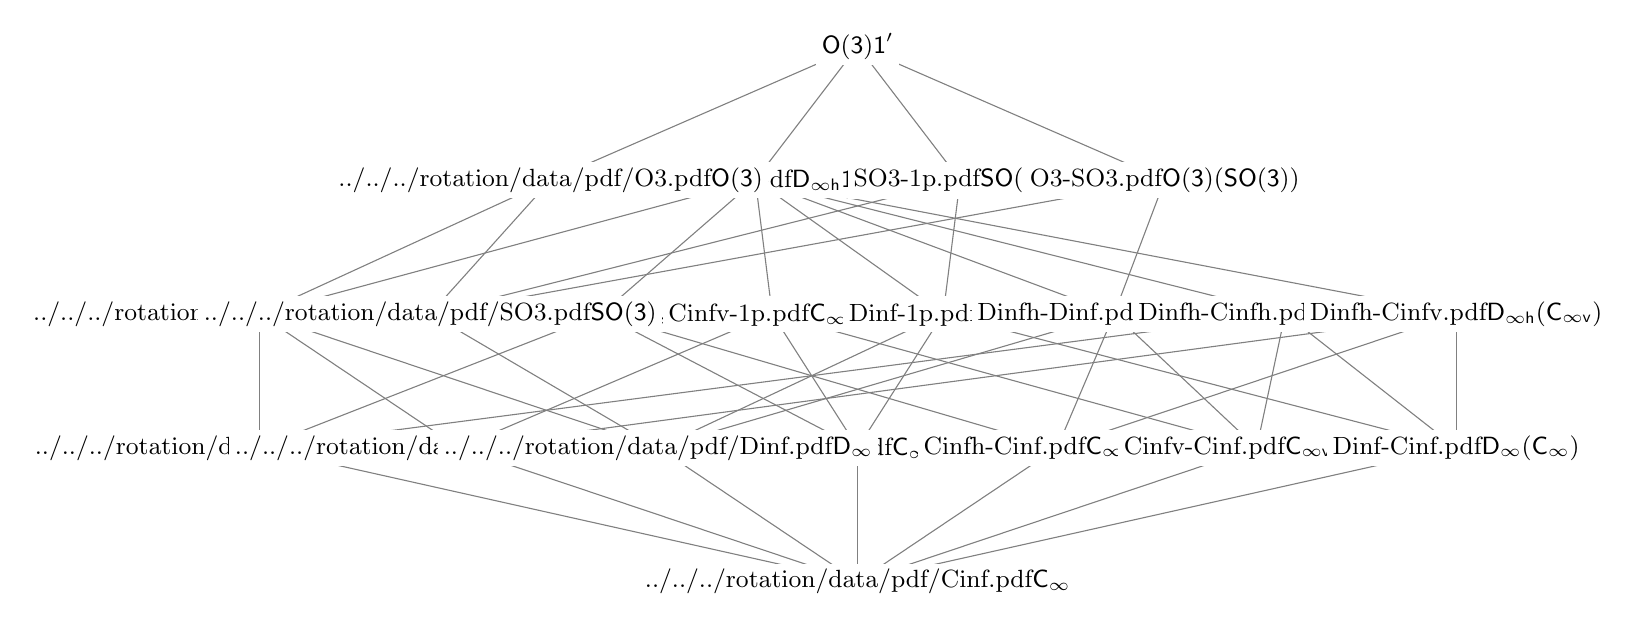
\begin{tikzpicture}[x=1cm, y=1cm, every node/.style={fill=white, font=\small, inner sep=2pt}]
\draw[black!50, line width=0.4pt] (0,0) -- (0,1.7);
\draw[black!50, line width=0.4pt] (0,0) -- (-7.6,1.7);
\draw[black!50, line width=0.4pt] (0,1.7) -- (-3.257,3.4);
\draw[black!50, line width=0.4pt] (-7.6,1.7) -- (-3.257,3.4);
\draw[black!50, line width=0.4pt] (2.533,1.7) -- (-3.257,3.4);
\draw[black!50, line width=0.4pt] (0,0) -- (2.533,1.7);
\draw[black!50, line width=0.4pt] (0,0) -- (-5.067,1.7);
\draw[black!50, line width=0.4pt] (0,1.7) -- (-1.086,3.4);
\draw[black!50, line width=0.4pt] (-5.067,1.7) -- (-1.086,3.4);
\draw[black!50, line width=0.4pt] (5.067,1.7) -- (-1.086,3.4);
\draw[black!50, line width=0.4pt] (0,0) -- (5.067,1.7);
\draw[black!50, line width=0.4pt] (0,0) -- (-2.533,1.7);
\draw[black!50, line width=0.4pt] (0,1.7) -- (1.086,3.4);
\draw[black!50, line width=0.4pt] (-2.533,1.7) -- (1.086,3.4);
\draw[black!50, line width=0.4pt] (7.6,1.7) -- (1.086,3.4);
\draw[black!50, line width=0.4pt] (0,0) -- (7.6,1.7);
\draw[black!50, line width=0.4pt] (-7.6,1.7) -- (-7.6,3.4);
\draw[black!50, line width=0.4pt] (-5.067,1.7) -- (-7.6,3.4);
\draw[black!50, line width=0.4pt] (-2.533,1.7) -- (-7.6,3.4);
\draw[black!50, line width=0.4pt] (-3.257,3.4) -- (-1.3,5.1);
\draw[black!50, line width=0.4pt] (-1.086,3.4) -- (-1.3,5.1);
\draw[black!50, line width=0.4pt] (1.086,3.4) -- (-1.3,5.1);
\draw[black!50, line width=0.4pt] (-7.6,3.4) -- (-1.3,5.1);
\draw[black!50, line width=0.4pt] (3.257,3.4) -- (-1.3,5.1);
\draw[black!50, line width=0.4pt] (5.429,3.4) -- (-1.3,5.1);
\draw[black!50, line width=0.4pt] (7.6,3.4) -- (-1.3,5.1);
\draw[black!50, line width=0.4pt] (2.533,1.7) -- (3.257,3.4);
\draw[black!50, line width=0.4pt] (5.067,1.7) -- (3.257,3.4);
\draw[black!50, line width=0.4pt] (-2.533,1.7) -- (3.257,3.4);
\draw[black!50, line width=0.4pt] (-7.6,1.7) -- (5.429,3.4);
\draw[black!50, line width=0.4pt] (5.067,1.7) -- (5.429,3.4);
\draw[black!50, line width=0.4pt] (7.6,1.7) -- (5.429,3.4);
\draw[black!50, line width=0.4pt] (2.533,1.7) -- (7.6,3.4);
\draw[black!50, line width=0.4pt] (-5.067,1.7) -- (7.6,3.4);
\draw[black!50, line width=0.4pt] (7.6,1.7) -- (7.6,3.4);
\draw[black!50, line width=0.4pt] (-2.533,1.7) -- (-5.429,3.4);
\draw[black!50, line width=0.4pt] (1.086,3.4) -- (1.3,5.1);
\draw[black!50, line width=0.4pt] (-5.429,3.4) -- (1.3,5.1);
\draw[black!50, line width=0.4pt] (-7.6,3.4) -- (-3.9,5.1);
\draw[black!50, line width=0.4pt] (-5.429,3.4) -- (-3.9,5.1);
\draw[black!50, line width=0.4pt] (3.257,3.4) -- (3.9,5.1);
\draw[black!50, line width=0.4pt] (-5.429,3.4) -- (3.9,5.1);
\draw[black!50, line width=0.4pt] (-1.3,5.1) -- (0,6.8);
\draw[black!50, line width=0.4pt] (1.3,5.1) -- (0,6.8);
\draw[black!50, line width=0.4pt] (-3.9,5.1) -- (0,6.8);
\draw[black!50, line width=0.4pt] (3.9,5.1) -- (0,6.8);
\node at (0,0) {\href{../../../rotation/data/pdf/Cinf.pdf}{\textcolor{black}{$\grp{C_{\infty}}$}}};
\node at (0,1.7) {\href{Cinf-1p.pdf}{\textcolor{black}{$\grp{C_{\infty}1'}$}}};
\node at (-7.6,1.7) {\href{../../../rotation/data/pdf/Cinfh.pdf}{\textcolor{black}{$\grp{C_{\infty h}}$}}};
\node at (-3.257,3.4) {\href{Cinfh-1p.pdf}{\textcolor{black}{$\grp{C_{\infty h}1'}$}}};
\node at (2.533,1.7) {\href{Cinfh-Cinf.pdf}{\textcolor{black}{$\grp{C_{\infty h}}(\grp{C_{\infty}})$}}};
\node at (-5.067,1.7) {\href{../../../rotation/data/pdf/Cinfv.pdf}{\textcolor{black}{$\grp{C_{\infty v}}$}}};
\node at (-1.086,3.4) {\href{Cinfv-1p.pdf}{\textcolor{black}{$\grp{C_{\infty v}1'}$}}};
\node at (5.067,1.7) {\href{Cinfv-Cinf.pdf}{\textcolor{black}{$\grp{C_{\infty v}}(\grp{C_{\infty}})$}}};
\node at (-2.533,1.7) {\href{../../../rotation/data/pdf/Dinf.pdf}{\textcolor{black}{$\grp{D_{\infty}}$}}};
\node at (1.086,3.4) {\href{Dinf-1p.pdf}{\textcolor{black}{$\grp{D_{\infty}1'}$}}};
\node at (7.6,1.7) {\href{Dinf-Cinf.pdf}{\textcolor{black}{$\grp{D_{\infty}}(\grp{C_{\infty}})$}}};
\node at (-7.6,3.4) {\href{../../../rotation/data/pdf/Dinfh.pdf}{\textcolor{black}{$\grp{D_{\infty h}}$}}};
\node at (-1.3,5.1) {\href{Dinfh-1p.pdf}{\textcolor{black}{$\grp{D_{\infty h}1'}$}}};
\node at (3.257,3.4) {\href{Dinfh-Dinf.pdf}{\textcolor{black}{$\grp{D_{\infty h}}(\grp{D_{\infty}})$}}};
\node at (5.429,3.4) {\href{Dinfh-Cinfh.pdf}{\textcolor{black}{$\grp{D_{\infty h}}(\grp{C_{\infty h}})$}}};
\node at (7.6,3.4) {\href{Dinfh-Cinfv.pdf}{\textcolor{black}{$\grp{D_{\infty h}}(\grp{C_{\infty v}})$}}};
\node at (-5.429,3.4) {\href{../../../rotation/data/pdf/SO3.pdf}{\textcolor{black}{$\grp{SO(3)}$}}};
\node at (1.3,5.1) {\href{SO3-1p.pdf}{\textcolor{black}{$\grp{SO(3)1'}$}}};
\node at (-3.9,5.1) {\href{../../../rotation/data/pdf/O3.pdf}{\textcolor{black}{$\grp{O(3)}$}}};
\node at (3.9,5.1) {\href{O3-SO3.pdf}{\textcolor{black}{$\grp{O(3)}(\grp{SO(3)})$}}};
\node at (0,6.8) {\textcolor{black}{$\grp{O(3)1'}$}};
\end{tikzpicture}\end{center}
The table lists the closed subgroups other than $\grp{O(3)1'}$ up to conjugacy in $\grp{O(3)1'}$, one in each row: the continuous subgroups, then those over the members of each family, then those over the exceptional groups. \label{n:index.family.N}A row with $N$ in its symbol stands for every $N$ of its range, and its entries are functions of $N$. \label{n:head.subgroup}\label{n:head.magnetic.type}\label{n:head.order}\label{n:head.conjugates}\label{n:head.normal}A row gives the representative of a class of subgroups (subgrp), its magnetic type (type), its order, the number of subgroups in the class (conjugates) and whether the representative is normal. \label{n:head.normalizer}\label{n:head.centralizer}It also gives its normalizer and its centralizer in $\grp{O(3)1'}$. The record holds the members with $N \le 12$ (\texttt{subgroup\symbol{95}classes}), and the section Closed subgroups of the document of \href{../../../rotation/data/pdf/O3.pdf}{$\grp{O(3)}$} gives other names of some members with $N = 1$.
{\small\begin{longtable}{@{}llrrlll@{}}\toprule
subgrp & type & order & conjugates & normal & normalizer & centralizer\\\midrule\endhead
\bottomrule\endfoot\endlastfoot
\href{../../../rotation/data/pdf/Cinf.pdf}{$\grp{C_{\infty}}$} & I & $\infty$ & $\infty$ & no & \href{Dinfh-1p.pdf}{$\grp{D_{\infty h}1'}$} & \href{Cinfh-1p.pdf}{$\grp{C_{\infty h}1'}$}\\*
\href{Cinf-1p.pdf}{$\grp{C_{\infty}1'}$} & II & $\infty$ & $\infty$ & no & \href{Dinfh-1p.pdf}{$\grp{D_{\infty h}1'}$} & \href{Cinfh-1p.pdf}{$\grp{C_{\infty h}1'}$}\\
\href{../../../rotation/data/pdf/Cinfh.pdf}{$\grp{C_{\infty h}}$} & I & $\infty$ & $\infty$ & no & \href{Dinfh-1p.pdf}{$\grp{D_{\infty h}1'}$} & \href{Cinfh-1p.pdf}{$\grp{C_{\infty h}1'}$}\\
\href{Cinfh-1p.pdf}{$\grp{C_{\infty h}1'}$} & II & $\infty$ & $\infty$ & no & \href{Dinfh-1p.pdf}{$\grp{D_{\infty h}1'}$} & \href{Cinfh-1p.pdf}{$\grp{C_{\infty h}1'}$}\\
\href{Cinfh-Cinf.pdf}{$\grp{C_{\infty h}}(\grp{C_{\infty}})$} & III & $\infty$ & $\infty$ & no & \href{Dinfh-1p.pdf}{$\grp{D_{\infty h}1'}$} & \href{Cinfh-1p.pdf}{$\grp{C_{\infty h}1'}$}\\
\href{../../../rotation/data/pdf/Cinfv.pdf}{$\grp{C_{\infty v}}$} & I & $\infty$ & $\infty$ & no & \href{Dinfh-1p.pdf}{$\grp{D_{\infty h}1'}$} & \href{C2h-1p.pdf}{$\grp{C_{2h}1'}$}\\
\href{Cinfv-1p.pdf}{$\grp{C_{\infty v}1'}$} & II & $\infty$ & $\infty$ & no & \href{Dinfh-1p.pdf}{$\grp{D_{\infty h}1'}$} & \href{C2h-1p.pdf}{$\grp{C_{2h}1'}$}\\
\href{Cinfv-Cinf.pdf}{$\grp{C_{\infty v}}(\grp{C_{\infty}})$} & III & $\infty$ & $\infty$ & no & \href{Dinfh-1p.pdf}{$\grp{D_{\infty h}1'}$} & \href{C2h-1p.pdf}{$\grp{C_{2h}1'}$}\\
\href{../../../rotation/data/pdf/Dinf.pdf}{$\grp{D_{\infty}}$} & I & $\infty$ & $\infty$ & no & \href{Dinfh-1p.pdf}{$\grp{D_{\infty h}1'}$} & \href{C2h-1p.pdf}{$\grp{C_{2h}1'}$}\\
\href{Dinf-1p.pdf}{$\grp{D_{\infty}1'}$} & II & $\infty$ & $\infty$ & no & \href{Dinfh-1p.pdf}{$\grp{D_{\infty h}1'}$} & \href{C2h-1p.pdf}{$\grp{C_{2h}1'}$}\\
\href{Dinf-Cinf.pdf}{$\grp{D_{\infty}}(\grp{C_{\infty}})$} & III & $\infty$ & $\infty$ & no & \href{Dinfh-1p.pdf}{$\grp{D_{\infty h}1'}$} & \href{C2h-1p.pdf}{$\grp{C_{2h}1'}$}\\
\href{../../../rotation/data/pdf/Dinfh.pdf}{$\grp{D_{\infty h}}$} & I & $\infty$ & $\infty$ & no & \href{Dinfh-1p.pdf}{$\grp{D_{\infty h}1'}$} & \href{C2h-1p.pdf}{$\grp{C_{2h}1'}$}\\
\href{Dinfh-1p.pdf}{$\grp{D_{\infty h}1'}$} & II & $\infty$ & $\infty$ & no & \href{Dinfh-1p.pdf}{$\grp{D_{\infty h}1'}$} & \href{C2h-1p.pdf}{$\grp{C_{2h}1'}$}\\
\href{Dinfh-Dinf.pdf}{$\grp{D_{\infty h}}(\grp{D_{\infty}})$} & III & $\infty$ & $\infty$ & no & \href{Dinfh-1p.pdf}{$\grp{D_{\infty h}1'}$} & \href{C2h-1p.pdf}{$\grp{C_{2h}1'}$}\\
\href{Dinfh-Cinfh.pdf}{$\grp{D_{\infty h}}(\grp{C_{\infty h}})$} & III & $\infty$ & $\infty$ & no & \href{Dinfh-1p.pdf}{$\grp{D_{\infty h}1'}$} & \href{C2h-1p.pdf}{$\grp{C_{2h}1'}$}\\
\href{Dinfh-Cinfv.pdf}{$\grp{D_{\infty h}}(\grp{C_{\infty v}})$} & III & $\infty$ & $\infty$ & no & \href{Dinfh-1p.pdf}{$\grp{D_{\infty h}1'}$} & \href{C2h-1p.pdf}{$\grp{C_{2h}1'}$}\\
\href{../../../rotation/data/pdf/SO3.pdf}{$\grp{SO(3)}$} & I & $\infty$ & 1 & yes & \href{O3-1p.pdf}{$\grp{O(3)1'}$} & \href{S2-1p.pdf}{$\grp{C_{i}1'}$}\\
\href{SO3-1p.pdf}{$\grp{SO(3)1'}$} & II & $\infty$ & 1 & yes & \href{O3-1p.pdf}{$\grp{O(3)1'}$} & \href{S2-1p.pdf}{$\grp{C_{i}1'}$}\\
\href{../../../rotation/data/pdf/O3.pdf}{$\grp{O(3)}$} & I & $\infty$ & 1 & yes & \href{O3-1p.pdf}{$\grp{O(3)1'}$} & \href{S2-1p.pdf}{$\grp{C_{i}1'}$}\\
\href{O3-SO3.pdf}{$\grp{O(3)}(\grp{SO(3)})$} & III & $\infty$ & 1 & yes & \href{O3-1p.pdf}{$\grp{O(3)1'}$} & \href{S2-1p.pdf}{$\grp{C_{i}1'}$}\\
\grouprule{0pt}{\lightrulewidth}
\href{../../../rotation/data/pdf/C1.pdf}{$\grp{C_{1}}$} & I & 1 & 1 & yes & \href{O3-1p.pdf}{$\grp{O(3)1'}$} & \href{O3-1p.pdf}{$\grp{O(3)1'}$}\\
\href{../../../rotation/data/pdf/C2.pdf}{$\grp{C_{2}}$} & I & 2 & $\infty$ & no & \href{Dinfh-1p.pdf}{$\grp{D_{\infty h}1'}$} & \href{Dinfh-1p.pdf}{$\grp{D_{\infty h}1'}$}\\
$\grp{C_{\mathnormal{N}}}$, $N \ge 3$ & I & $N$ & $\infty$ & no & \href{Dinfh-1p.pdf}{$\grp{D_{\infty h}1'}$} & \href{Cinfh-1p.pdf}{$\grp{C_{\infty h}1'}$}\\
\href{C1-1p.pdf}{$\grp{C_{1}1'}$} & II & 2 & 1 & yes & \href{O3-1p.pdf}{$\grp{O(3)1'}$} & \href{O3-1p.pdf}{$\grp{O(3)1'}$}\\
\href{C2-1p.pdf}{$\grp{C_{2}1'}$} & II & 4 & $\infty$ & no & \href{Dinfh-1p.pdf}{$\grp{D_{\infty h}1'}$} & \href{Dinfh-1p.pdf}{$\grp{D_{\infty h}1'}$}\\
$\grp{C_{\mathnormal{N}}1'}$, $N \ge 3$ & II & $2N$ & $\infty$ & no & \href{Dinfh-1p.pdf}{$\grp{D_{\infty h}1'}$} & \href{Cinfh-1p.pdf}{$\grp{C_{\infty h}1'}$}\\
\href{C2-C1.pdf}{$\grp{C_{2}}(\grp{C_{1}})$} & III & 2 & $\infty$ & no & \href{Dinfh-1p.pdf}{$\grp{D_{\infty h}1'}$} & \href{Dinfh-1p.pdf}{$\grp{D_{\infty h}1'}$}\\
$\grp{C_{2\mathnormal{N}}}(\grp{C_{\mathnormal{N}}})$, $N \ge 2$ & III & $2N$ & $\infty$ & no & \href{Dinfh-1p.pdf}{$\grp{D_{\infty h}1'}$} & \href{Cinfh-1p.pdf}{$\grp{C_{\infty h}1'}$}\\
\grouprule{0pt}{\lightrulewidth}
\href{../../../rotation/data/pdf/S2.pdf}{$\grp{C_{i}}$} & I & 2 & 1 & yes & \href{O3-1p.pdf}{$\grp{O(3)1'}$} & \href{O3-1p.pdf}{$\grp{O(3)1'}$}\\
$\grp{S_{2\mathnormal{N}}}$, $N \ge 2$ & I & $2N$ & $\infty$ & no & \href{Dinfh-1p.pdf}{$\grp{D_{\infty h}1'}$} & \href{Cinfh-1p.pdf}{$\grp{C_{\infty h}1'}$}\\
\href{S2-1p.pdf}{$\grp{C_{i}1'}$} & II & 4 & 1 & yes & \href{O3-1p.pdf}{$\grp{O(3)1'}$} & \href{O3-1p.pdf}{$\grp{O(3)1'}$}\\
$\grp{S_{2\mathnormal{N}}1'}$, $N \ge 2$ & II & $4N$ & $\infty$ & no & \href{Dinfh-1p.pdf}{$\grp{D_{\infty h}1'}$} & \href{Cinfh-1p.pdf}{$\grp{C_{\infty h}1'}$}\\
\href{S2-C1.pdf}{$\grp{C_{i}}(\grp{C_{1}})$} & III & 2 & 1 & yes & \href{O3-1p.pdf}{$\grp{O(3)1'}$} & \href{O3-1p.pdf}{$\grp{O(3)1'}$}\\
$\grp{S_{2\mathnormal{N}}}(\grp{C_{\mathnormal{N}}})$, $N \ge 2$ & III & $2N$ & $\infty$ & no & \href{Dinfh-1p.pdf}{$\grp{D_{\infty h}1'}$} & \href{Cinfh-1p.pdf}{$\grp{C_{\infty h}1'}$}\\
\grouprule{0pt}{\lightrulewidth}
\href{../../../rotation/data/pdf/C2h.pdf}{$\grp{C_{2h}}$} & I & 4 & $\infty$ & no & \href{Dinfh-1p.pdf}{$\grp{D_{\infty h}1'}$} & \href{Dinfh-1p.pdf}{$\grp{D_{\infty h}1'}$}\\
$\grp{C_{\mathnormal{N}h}}$, $N \ge 3$ & I & $2N$ & $\infty$ & no & \href{Dinfh-1p.pdf}{$\grp{D_{\infty h}1'}$} & \href{Cinfh-1p.pdf}{$\grp{C_{\infty h}1'}$}\\
\href{C2h-1p.pdf}{$\grp{C_{2h}1'}$} & II & 8 & $\infty$ & no & \href{Dinfh-1p.pdf}{$\grp{D_{\infty h}1'}$} & \href{Dinfh-1p.pdf}{$\grp{D_{\infty h}1'}$}\\
$\grp{C_{\mathnormal{N}h}1'}$, $N \ge 3$ & II & $4N$ & $\infty$ & no & \href{Dinfh-1p.pdf}{$\grp{D_{\infty h}1'}$} & \href{Cinfh-1p.pdf}{$\grp{C_{\infty h}1'}$}\\
\href{C2h-C2.pdf}{$\grp{C_{2h}}(\grp{C_{2}})$} & III & 4 & $\infty$ & no & \href{Dinfh-1p.pdf}{$\grp{D_{\infty h}1'}$} & \href{Dinfh-1p.pdf}{$\grp{D_{\infty h}1'}$}\\
$\grp{C_{\mathnormal{N}h}}(\grp{C_{\mathnormal{N}}})$, $N \ge 3$ & III & $2N$ & $\infty$ & no & \href{Dinfh-1p.pdf}{$\grp{D_{\infty h}1'}$} & \href{Cinfh-1p.pdf}{$\grp{C_{\infty h}1'}$}\\
\href{C2h-S2.pdf}{$\grp{C_{2h}}(\grp{C_{i}})$} & III & 4 & $\infty$ & no & \href{Dinfh-1p.pdf}{$\grp{D_{\infty h}1'}$} & \href{Dinfh-1p.pdf}{$\grp{D_{\infty h}1'}$}\\
$\grp{C_{2\mathnormal{N}h}}(\grp{S_{2\mathnormal{N}}})$, $N \ge 2$ & III & $4N$ & $\infty$ & no & \href{Dinfh-1p.pdf}{$\grp{D_{\infty h}1'}$} & \href{Cinfh-1p.pdf}{$\grp{C_{\infty h}1'}$}\\
\href{C2h-C1v.pdf}{$\grp{C_{2h}}(\grp{C_{s}})$} & III & 4 & $\infty$ & no & \href{Dinfh-1p.pdf}{$\grp{D_{\infty h}1'}$} & \href{Dinfh-1p.pdf}{$\grp{D_{\infty h}1'}$}\\
$\grp{C_{2\mathnormal{N}h}}(\grp{C_{\mathnormal{N}h}})$, $N \ge 2$ & III & $4N$ & $\infty$ & no & \href{Dinfh-1p.pdf}{$\grp{D_{\infty h}1'}$} & \href{Cinfh-1p.pdf}{$\grp{C_{\infty h}1'}$}\\
\grouprule{0pt}{\lightrulewidth}
\href{../../../rotation/data/pdf/C1v.pdf}{$\grp{C_{s}}$} & I & 2 & $\infty$ & no & \href{Dinfh-1p.pdf}{$\grp{D_{\infty h}1'}$} & \href{Dinfh-1p.pdf}{$\grp{D_{\infty h}1'}$}\\
\href{../../../rotation/data/pdf/C2v.pdf}{$\grp{C_{2v}}$} & I & 4 & $\infty$ & no & \href{D4h-1p.pdf}{$\grp{D_{4h}1'}$} & \href{D2h-1p.pdf}{$\grp{D_{2h}1'}$}\\
$\grp{C_{\mathnormal{N}v}}$, $N \ge 3$ & I & $2N$ & $\infty$ & no & $\grp{D_{2\mathnormal{N}h}1'}$ & \href{C2h-1p.pdf}{$\grp{C_{2h}1'}$}\\
\href{C1v-1p.pdf}{$\grp{C_{s}1'}$} & II & 4 & $\infty$ & no & \href{Dinfh-1p.pdf}{$\grp{D_{\infty h}1'}$} & \href{Dinfh-1p.pdf}{$\grp{D_{\infty h}1'}$}\\
\href{C2v-1p.pdf}{$\grp{C_{2v}1'}$} & II & 8 & $\infty$ & no & \href{D4h-1p.pdf}{$\grp{D_{4h}1'}$} & \href{D2h-1p.pdf}{$\grp{D_{2h}1'}$}\\
$\grp{C_{\mathnormal{N}v}1'}$, $N \ge 3$ & II & $4N$ & $\infty$ & no & $\grp{D_{2\mathnormal{N}h}1'}$ & \href{C2h-1p.pdf}{$\grp{C_{2h}1'}$}\\
\href{C1v-C1.pdf}{$\grp{C_{s}}(\grp{C_{1}})$} & III & 2 & $\infty$ & no & \href{Dinfh-1p.pdf}{$\grp{D_{\infty h}1'}$} & \href{Dinfh-1p.pdf}{$\grp{D_{\infty h}1'}$}\\
\href{C2v-C2.pdf}{$\grp{C_{2v}}(\grp{C_{2}})$} & III & 4 & $\infty$ & no & \href{D4h-1p.pdf}{$\grp{D_{4h}1'}$} & \href{D2h-1p.pdf}{$\grp{D_{2h}1'}$}\\
$\grp{C_{\mathnormal{N}v}}(\grp{C_{\mathnormal{N}}})$, $N \ge 3$ & III & $2N$ & $\infty$ & no & $\grp{D_{2\mathnormal{N}h}1'}$ & \href{C2h-1p.pdf}{$\grp{C_{2h}1'}$}\\
\href{C2v-C1v.pdf}{$\grp{C_{2v}}(\grp{C_{s}})$} & III & 4 & $\infty$ & no & \href{D2h-1p.pdf}{$\grp{D_{2h}1'}$} & \href{D2h-1p.pdf}{$\grp{D_{2h}1'}$}\\
$\grp{C_{2\mathnormal{N}v}}(\grp{C_{\mathnormal{N}v}})$, $N \ge 2$ & III & $4N$ & $\infty$ & no & $\grp{D_{2\mathnormal{N}h}1'}$ & \href{C2h-1p.pdf}{$\grp{C_{2h}1'}$}\\
\grouprule{0pt}{\lightrulewidth}
\href{../../../rotation/data/pdf/D2.pdf}{$\grp{D_{2}}$} & I & 4 & $\infty$ & no & \href{Oh-1p.pdf}{$\grp{O_{h}1'}$} & \href{D2h-1p.pdf}{$\grp{D_{2h}1'}$}\\
$\grp{D_{\mathnormal{N}}}$, $N \ge 3$ & I & $2N$ & $\infty$ & no & $\grp{D_{2\mathnormal{N}h}1'}$ & \href{C2h-1p.pdf}{$\grp{C_{2h}1'}$}\\
\href{D2-1p.pdf}{$\grp{D_{2}1'}$} & II & 8 & $\infty$ & no & \href{Oh-1p.pdf}{$\grp{O_{h}1'}$} & \href{D2h-1p.pdf}{$\grp{D_{2h}1'}$}\\
$\grp{D_{\mathnormal{N}}1'}$, $N \ge 3$ & II & $4N$ & $\infty$ & no & $\grp{D_{2\mathnormal{N}h}1'}$ & \href{C2h-1p.pdf}{$\grp{C_{2h}1'}$}\\
\href{D2-C2.pdf}{$\grp{D_{2}}(\grp{C_{2}})$} & III & 4 & $\infty$ & no & \href{D4h-1p.pdf}{$\grp{D_{4h}1'}$} & \href{D2h-1p.pdf}{$\grp{D_{2h}1'}$}\\
$\grp{D_{\mathnormal{N}}}(\grp{C_{\mathnormal{N}}})$, $N \ge 3$ & III & $2N$ & $\infty$ & no & $\grp{D_{2\mathnormal{N}h}1'}$ & \href{C2h-1p.pdf}{$\grp{C_{2h}1'}$}\\
$\grp{D_{2\mathnormal{N}}}(\grp{D_{\mathnormal{N}}})$, $N \ge 2$ & III & $4N$ & $\infty$ & no & $\grp{D_{2\mathnormal{N}h}1'}$ & \href{C2h-1p.pdf}{$\grp{C_{2h}1'}$}\\
\grouprule{0pt}{\lightrulewidth}
\href{../../../rotation/data/pdf/D2h.pdf}{$\grp{D_{2h}}$} & I & 8 & $\infty$ & no & \href{Oh-1p.pdf}{$\grp{O_{h}1'}$} & \href{D2h-1p.pdf}{$\grp{D_{2h}1'}$}\\
$\grp{D_{\mathnormal{N}h}}$, $N \ge 3$ & I & $4N$ & $\infty$ & no & $\grp{D_{2\mathnormal{N}h}1'}$ & \href{C2h-1p.pdf}{$\grp{C_{2h}1'}$}\\
\href{D2h-1p.pdf}{$\grp{D_{2h}1'}$} & II & 16 & $\infty$ & no & \href{Oh-1p.pdf}{$\grp{O_{h}1'}$} & \href{D2h-1p.pdf}{$\grp{D_{2h}1'}$}\\
$\grp{D_{\mathnormal{N}h}1'}$, $N \ge 3$ & II & $8N$ & $\infty$ & no & $\grp{D_{2\mathnormal{N}h}1'}$ & \href{C2h-1p.pdf}{$\grp{C_{2h}1'}$}\\
\href{D2h-D2.pdf}{$\grp{D_{2h}}(\grp{D_{2}})$} & III & 8 & $\infty$ & no & \href{Oh-1p.pdf}{$\grp{O_{h}1'}$} & \href{D2h-1p.pdf}{$\grp{D_{2h}1'}$}\\
$\grp{D_{\mathnormal{N}h}}(\grp{D_{\mathnormal{N}}})$, $N \ge 3$ & III & $4N$ & $\infty$ & no & $\grp{D_{2\mathnormal{N}h}1'}$ & \href{C2h-1p.pdf}{$\grp{C_{2h}1'}$}\\
\href{D2h-C2h.pdf}{$\grp{D_{2h}}(\grp{C_{2h}})$} & III & 8 & $\infty$ & no & \href{D4h-1p.pdf}{$\grp{D_{4h}1'}$} & \href{D2h-1p.pdf}{$\grp{D_{2h}1'}$}\\
$\grp{D_{\mathnormal{N}h}}(\grp{C_{\mathnormal{N}h}})$, $N \ge 3$ & III & $4N$ & $\infty$ & no & $\grp{D_{2\mathnormal{N}h}1'}$ & \href{C2h-1p.pdf}{$\grp{C_{2h}1'}$}\\
\href{D2h-C2v.pdf}{$\grp{D_{2h}}(\grp{C_{2v}})$} & III & 8 & $\infty$ & no & \href{D4h-1p.pdf}{$\grp{D_{4h}1'}$} & \href{D2h-1p.pdf}{$\grp{D_{2h}1'}$}\\
$\grp{D_{\mathnormal{N}h}}(\grp{C_{\mathnormal{N}v}})$, $N \ge 3$ & III & $4N$ & $\infty$ & no & $\grp{D_{2\mathnormal{N}h}1'}$ & \href{C2h-1p.pdf}{$\grp{C_{2h}1'}$}\\
$\grp{D_{2\mathnormal{N}h}}(\grp{D_{\mathnormal{N}h}})$, $N \ge 2$ & III & $8N$ & $\infty$ & no & $\grp{D_{2\mathnormal{N}h}1'}$ & \href{C2h-1p.pdf}{$\grp{C_{2h}1'}$}\\
$\grp{D_{2\mathnormal{N}h}}(\grp{D_{\mathnormal{N}d}})$, $N \ge 2$ & III & $8N$ & $\infty$ & no & $\grp{D_{2\mathnormal{N}h}1'}$ & \href{C2h-1p.pdf}{$\grp{C_{2h}1'}$}\\
\grouprule{0pt}{\lightrulewidth}
$\grp{D_{\mathnormal{N}d}}$, $N \ge 2$ & I & $4N$ & $\infty$ & no & $\grp{D_{2\mathnormal{N}h}1'}$ & \href{C2h-1p.pdf}{$\grp{C_{2h}1'}$}\\
$\grp{D_{\mathnormal{N}d}1'}$, $N \ge 2$ & II & $8N$ & $\infty$ & no & $\grp{D_{2\mathnormal{N}h}1'}$ & \href{C2h-1p.pdf}{$\grp{C_{2h}1'}$}\\
$\grp{D_{\mathnormal{N}d}}(\grp{D_{\mathnormal{N}}})$, $N \ge 2$ & III & $4N$ & $\infty$ & no & $\grp{D_{2\mathnormal{N}h}1'}$ & \href{C2h-1p.pdf}{$\grp{C_{2h}1'}$}\\
$\grp{D_{\mathnormal{N}d}}(\grp{S_{2\mathnormal{N}}})$, $N \ge 2$ & III & $4N$ & $\infty$ & no & $\grp{D_{2\mathnormal{N}h}1'}$ & \href{C2h-1p.pdf}{$\grp{C_{2h}1'}$}\\
$\grp{D_{\mathnormal{N}d}}(\grp{C_{\mathnormal{N}v}})$, $N \ge 2$ & III & $4N$ & $\infty$ & no & $\grp{D_{2\mathnormal{N}h}1'}$ & \href{C2h-1p.pdf}{$\grp{C_{2h}1'}$}\\
\grouprule{0pt}{\lightrulewidth}
\href{../../../rotation/data/pdf/T.pdf}{$\grp{T}$} & I & 12 & $\infty$ & no & \href{Oh-1p.pdf}{$\grp{O_{h}1'}$} & \href{S2-1p.pdf}{$\grp{C_{i}1'}$}\\
\href{T-1p.pdf}{$\grp{T1'}$} & II & 24 & $\infty$ & no & \href{Oh-1p.pdf}{$\grp{O_{h}1'}$} & \href{S2-1p.pdf}{$\grp{C_{i}1'}$}\\
\href{../../../rotation/data/pdf/Th.pdf}{$\grp{T_{h}}$} & I & 24 & $\infty$ & no & \href{Oh-1p.pdf}{$\grp{O_{h}1'}$} & \href{S2-1p.pdf}{$\grp{C_{i}1'}$}\\
\href{Th-1p.pdf}{$\grp{T_{h}1'}$} & II & 48 & $\infty$ & no & \href{Oh-1p.pdf}{$\grp{O_{h}1'}$} & \href{S2-1p.pdf}{$\grp{C_{i}1'}$}\\
\href{Th-T.pdf}{$\grp{T_{h}}(\grp{T})$} & III & 24 & $\infty$ & no & \href{Oh-1p.pdf}{$\grp{O_{h}1'}$} & \href{S2-1p.pdf}{$\grp{C_{i}1'}$}\\
\href{../../../rotation/data/pdf/Td.pdf}{$\grp{T_{d}}$} & I & 24 & $\infty$ & no & \href{Oh-1p.pdf}{$\grp{O_{h}1'}$} & \href{S2-1p.pdf}{$\grp{C_{i}1'}$}\\
\href{Td-1p.pdf}{$\grp{T_{d}1'}$} & II & 48 & $\infty$ & no & \href{Oh-1p.pdf}{$\grp{O_{h}1'}$} & \href{S2-1p.pdf}{$\grp{C_{i}1'}$}\\
\href{Td-T.pdf}{$\grp{T_{d}}(\grp{T})$} & III & 24 & $\infty$ & no & \href{Oh-1p.pdf}{$\grp{O_{h}1'}$} & \href{S2-1p.pdf}{$\grp{C_{i}1'}$}\\
\href{../../../rotation/data/pdf/O.pdf}{$\grp{O}$} & I & 24 & $\infty$ & no & \href{Oh-1p.pdf}{$\grp{O_{h}1'}$} & \href{S2-1p.pdf}{$\grp{C_{i}1'}$}\\
\href{O-1p.pdf}{$\grp{O1'}$} & II & 48 & $\infty$ & no & \href{Oh-1p.pdf}{$\grp{O_{h}1'}$} & \href{S2-1p.pdf}{$\grp{C_{i}1'}$}\\
\href{O-T.pdf}{$\grp{O}(\grp{T})$} & III & 24 & $\infty$ & no & \href{Oh-1p.pdf}{$\grp{O_{h}1'}$} & \href{S2-1p.pdf}{$\grp{C_{i}1'}$}\\
\href{../../../rotation/data/pdf/Oh.pdf}{$\grp{O_{h}}$} & I & 48 & $\infty$ & no & \href{Oh-1p.pdf}{$\grp{O_{h}1'}$} & \href{S2-1p.pdf}{$\grp{C_{i}1'}$}\\
\href{Oh-1p.pdf}{$\grp{O_{h}1'}$} & II & 96 & $\infty$ & no & \href{Oh-1p.pdf}{$\grp{O_{h}1'}$} & \href{S2-1p.pdf}{$\grp{C_{i}1'}$}\\
\href{Oh-O.pdf}{$\grp{O_{h}}(\grp{O})$} & III & 48 & $\infty$ & no & \href{Oh-1p.pdf}{$\grp{O_{h}1'}$} & \href{S2-1p.pdf}{$\grp{C_{i}1'}$}\\
\href{Oh-Th.pdf}{$\grp{O_{h}}(\grp{T_{h}})$} & III & 48 & $\infty$ & no & \href{Oh-1p.pdf}{$\grp{O_{h}1'}$} & \href{S2-1p.pdf}{$\grp{C_{i}1'}$}\\
\href{Oh-Td.pdf}{$\grp{O_{h}}(\grp{T_{d}})$} & III & 48 & $\infty$ & no & \href{Oh-1p.pdf}{$\grp{O_{h}1'}$} & \href{S2-1p.pdf}{$\grp{C_{i}1'}$}\\
\href{../../../rotation/data/pdf/I.pdf}{$\grp{I}$} & I & 60 & $\infty$ & no & \href{Ih-1p.pdf}{$\grp{I_{h}1'}$} & \href{S2-1p.pdf}{$\grp{C_{i}1'}$}\\
\href{I-1p.pdf}{$\grp{I1'}$} & II & 120 & $\infty$ & no & \href{Ih-1p.pdf}{$\grp{I_{h}1'}$} & \href{S2-1p.pdf}{$\grp{C_{i}1'}$}\\
\href{../../../rotation/data/pdf/Ih.pdf}{$\grp{I_{h}}$} & I & 120 & $\infty$ & no & \href{Ih-1p.pdf}{$\grp{I_{h}1'}$} & \href{S2-1p.pdf}{$\grp{C_{i}1'}$}\\
\href{Ih-1p.pdf}{$\grp{I_{h}1'}$} & II & 240 & $\infty$ & no & \href{Ih-1p.pdf}{$\grp{I_{h}1'}$} & \href{S2-1p.pdf}{$\grp{C_{i}1'}$}\\*
\href{Ih-I.pdf}{$\grp{I_{h}}(\grp{I})$} & III & 120 & $\infty$ & no & \href{Ih-1p.pdf}{$\grp{I_{h}1'}$} & \href{S2-1p.pdf}{$\grp{C_{i}1'}$}\\
\bottomrule\end{longtable}}
\needspace{190pt}
\partbox{Angular momentum}
\section{Subduction from \texorpdfstring{$\grp{O(3)1'}$}{O(3)1\unichar{8242}}}\label{s:subduction_o3}
Conventions: \href{../../CONVENTIONS.pdf}{CONVENTIONS.pdf}, sections \href{../../../rotation/CONVENTIONS.pdf\#conv.11}{11}, \href{../../../rotation/CONVENTIONS.pdf\#conv.12}{12}, \href{../../CONVENTIONS.pdf\#conv.33.1}{33.1} and \href{../../CONVENTIONS.pdf\#conv.37.4}{37.4}.
\leavevmode\label{n:index.J}\label{n:index.parity}The irrep $\irrJp{J}{p}$ of $\grp{O(3)1'}$ has angular momentum $J$ and parity $p$ ($\ptag{g}$ for $p = +1$, $\ptag{u}$ for $p = -1$), and time reversal acts on it as on its kets (\href{../../CONVENTIONS.pdf}{CONVENTIONS.pdf}, section \href{../../CONVENTIONS.pdf\#conv.31.1}{31.1}). A corepresentation occurs in its restriction to $\grp{O(3)1'}$ as often as its first irrep occurs in the restriction to $\grp{O(3)}$ (the section Subduction from $\grp{O(3)}$ of the document of \href{../../../rotation/data/pdf/O3.pdf}{$\grp{O(3)}$}). For every $J$,
\begin{equation}\label{e:o3rule}\restr{\irrJp{J}{p}}{\grp{O(3)1'}} = \irrJp{J}{p}.\end{equation}
The record also holds the restrictions for $J \le 6$ (\texttt{subduction\symbol{95}corepresentations}).
\needspace{281pt}
\partbox{Tensors}
\section{Multipoles}\label{s:multipoles}
Conventions: \href{../../CONVENTIONS.pdf}{CONVENTIONS.pdf}, sections \href{../../CONVENTIONS.pdf\#conv.35.1}{35.1} and \href{../../CONVENTIONS.pdf\#conv.37.6}{37.6}.
A row is a rank $J$, and the last row gives every rank (\texttt{every\symbol{95}rank}). \label{n:head.multipole.electric}\label{n:head.multipole.electric.toroidal}A row gives the number of independent multipoles of each kind that $\grp{O(3)1'}$ allows. It is the multiplicity in $\irrJp{J}{p}$ of the trivial irrep of $\grp{O(3)}$ (the section Subduction from $\grp{O(3)}$ of the document of \href{../../../rotation/data/pdf/O3.pdf}{$\grp{O(3)}$}).
{\small\begin{longtable}{@{}rrr@{}}\toprule
$J$ & electric & electric toroidal\\\midrule\endhead
\bottomrule\endfoot\endlastfoot
0 & 1 & 0\\*
1 & 0 & 0\\*
2 & 0 & 0\\*
3 & 0 & 0\\*
4 & 0 & 0\\*
\grouprule{0pt}{\lightrulewidth} every & 1 for $J = 0$ & 0\\
\bottomrule\end{longtable}}
The electric entries at even $J$ count the operators on a spin that $\grp{O(3)1'}$ allows (\href{../../CONVENTIONS.pdf}{CONVENTIONS.pdf}, section \href{../../CONVENTIONS.pdf\#conv.35.1}{35.1}).
\needspace{103pt}
\section{Invariants}\label{s:invariants}
Conventions: \href{../../CONVENTIONS.pdf}{CONVENTIONS.pdf}, sections \href{../../CONVENTIONS.pdf\#conv.31.2}{31.2} and \href{../../CONVENTIONS.pdf\#conv.35.1}{35.1}.
The invariant polynomials of $\grp{O(3)1'}$ in one vector of a kind are those of its image of that kind (section~\ref{s:identification}), in the section Invariant polynomials of the image's document (\texttt{rings}).
\leavevmode\label{n:index.degree.polar}\label{n:index.degree.axial}A row is a degree $a$ in a polar vector even under time reversal. A row gives the number of linearly independent invariants of degree $a$ in it and $b$ in an axial vector odd under time reversal, for $a + b \le 6$.
{\small\begin{longtable}{@{}rrrrrr@{}}\toprule
$a$ & $b = 1$ & $b = 2$ & $b = 3$ & $b = 4$ & $b = 5$\\\midrule\endhead
\bottomrule\endfoot\endlastfoot
1 & 0 & 0 & 0 & 0 & 0\\*
2 & 0 & 2 & 0 & 2 & \\*
3 & 0 & 0 & 0 &  & \\*
4 & 0 & 2 &  &  & \\*
5 & 0 &  &  &  & \\
\bottomrule\end{longtable}}
\leavevmode\label{n:local.component.polar}\label{n:local.component.axial}The record holds their bases for $a + b \le 4$ (\texttt{polynomials}), in the components $u_{x}$, $u_{y}$, $u_{z}$ of the polar vector and $v_{x}$, $v_{y}$, $v_{z}$ of the axial vector. \label{n:head.polynomial}A row is an invariant of the reduced row echelon basis of its degrees (\href{../../CONVENTIONS.pdf}{CONVENTIONS.pdf}, section \href{../../CONVENTIONS.pdf\#conv.35.1}{35.1}). A row gives its degrees $a$ and $b$ and the invariant (polynomial).
{\small\renewcommand{\arraystretch}{1.2}\begin{longtable}{@{}rrl@{}}\toprule
$a$ & $b$ & polynomial\\\midrule\endhead
\bottomrule\endfoot\endlastfoot
2 & 2 & $u_{x}^{2}v_{x}^{2} + 2u_{x}u_{y}v_{x}v_{y} + 2u_{x}u_{z}v_{x}v_{z} + u_{y}^{2}v_{y}^{2} + 2u_{y}u_{z}v_{y}v_{z} + u_{z}^{2}v_{z}^{2}$\\*
2 & 2 & $u_{x}^{2}v_{y}^{2} + u_{x}^{2}v_{z}^{2} - 2u_{x}u_{y}v_{x}v_{y} - 2u_{x}u_{z}v_{x}v_{z} + u_{y}^{2}v_{x}^{2} + u_{y}^{2}v_{z}^{2} - 2u_{y}u_{z}v_{y}v_{z} + u_{z}^{2}v_{x}^{2} + u_{z}^{2}v_{y}^{2}$\\
\bottomrule\end{longtable}}
\end{document}
